\chapter{应用程序设计}

\section{开发及运行环境介绍}

系统采用前后端分离方式设计。前端使用vue框架实现,后端基于python的flask框架编写。

本地将前端和后端服务开启后,即可通过本地浏览器访问。若将服务部署到公网上,即可在外网通过ip地址访问该网页。

\section{后端设计}

\subsection{连接数据库}

下面的代码包含后端导入的python模块以及通过pymysql连接数据库的代码。其中, `config.json' 包含数据库连接的用户名等相关信息。

\scriptsize
\begin{minted}[linenos,breaklines]{python}
from flask import Flask, Response, request
import pymysql as sql
import json
from flask_cors import CORS
app = Flask(__name__)
CORS(app, supports_credentials=True)
app.config.from_json('config.json')
db = sql.connect(host=app.config["DB_HOST"],
                 user=app.config["DB_USER"],
                 password=app.config["DB_PASSWORD"],
                 db=app.config["DB_NAME"])
\end{minted}
\normalsize

\subsection{后端接口设计}

数据库中已经包含了所需的所有视图,因此查询数据时只要查询对应视图(并辅以排序和筛选等操作),而不用关心内部逻辑,从而简化后端查询的复杂度。

下面以SOTA查询接口为例,解释后端接口的工作方式。

\scriptsize
\begin{minted}[linenos,breaklines]{python}
@app.route('/sota', methods=['GET', 'POST'])
def sota():
    cur = db.cursor()
    cur.execute("SELECT * FROM v_task_papercount JOIN v_task_benchcount USING(taskId) ORDER BY paperCnt DESC;")
    results = cur.fetchall()
    lst = []
    for row in results:
        lst.append({
            "taskId": row[0],
            "taskName": row[1],
            "taskDesc": row[2],
            "paperCnt": row[3],
            "benchCnt": row[4]
        })
    cur.close()
    return Response(json.dumps(lst), mimetype='application/json')
\end{minted}
\normalsize

该函数获取了一个数据库的游标,并执行了一个查询。通过游标遍历查询结果,将结果组织为一个python字典。最后,转化为json格式,作为函数返回值传出。

后端也支持参数化查询,通过request.args.get获得前端传来的参数。下面是主页的后端查询接口:

\scriptsize
\begin{minted}[linenos,breaklines]{python}
@app.route('/paper', methods=['GET', 'POST'])
def paper():
    cur = db.cursor()
    order = "ORDER BY publishDate DESC"
    if request.args.get('order') == "star":
        order = "ORDER BY star DESC"
    cur.execute("SELECT * FROM v_paperstar WHERE title LIKE %s {}".format(order),
                ('%' + request.args.get('title') + '%')
                )
    results = cur.fetchall()
    lst = []
    for row in results:
        with db.cursor() as cur2:
            cur2.execute("SELECT authorName FROM v_author_of_paper WHERE paperId=%s AND ORD=1", (row[0]))
            lst.append({
                "id": row[0],
                "title": row[1],
                "paperLink": row[2],
                "abs": row[3],
                "publishDate": row[4].strftime('%Y-%m-%d'),
                "star": int(row[5]),
                "author": cur2.fetchone()[0]
            })
    cur.close()
    return Response(json.dumps(lst), mimetype='application/json')
\end{minted}
\normalsize

在上面的查询中,前端参数order控制查询的排序逻辑,参数title用于模糊查找。该项目中所有模糊查找均通过字符串的子串匹配(即查询条件中的LIKE)实现。

上面的代码中,cur.execute()的调用方式和java中的preparedStatement类似,是预编译好的,可以防止SQL注入。

\section{前端设计}

\subsection{核心组件}
前端通过vue框架实现。核心组件为router。前端的所有功能都需要在router中注册(在router/index.js中添加相关定义)。

\scriptsize
\begin{minted}[linenos,breaklines]{js}
import Vue from 'vue'
import Router from 'vue-router'
import Paper from '@/components/Paper'
import SOTA from '@/components/SOTA'
import Method from '@/components/Method'
import Task from '@/components/Task'
import Datasets from '@/components/Datasets'
import Author from '@/components/Author'
import Bench from '@/components/Bench'
import Dataset from '@/components/Dataset'
import Methods from "@/components/Methods";
import PaperInfo from "@/components/PaperInfo";

Vue.use(Router)

export default new Router({
  routes: [
    {
      path: '/',
      name: 'Paper',
      component: Paper,
    },
    {
      path: '/sota',
      name: 'SOTA',
      component: SOTA,
    },
    {
      path: '/methods',
      name: 'Methods',
      component: Methods,
    },
    {
      path: '/method',
      name: 'Method',
      component: Method,
    },
    {
      path: '/tasks',
      name: 'Tasks',
      component: Task,
    },
    {
      path: '/datasets',
      name: 'Datasets',
      component: Datasets,
    },
    {
      path: '/author',
      name: 'Author',
      component: Author,
    },
    {
      path: '/bench',
      name: 'Bench',
      component: Bench,
    },
    {
      path: '/dataset',
      name: 'Dataset',
      component: Dataset,
    },
    {
      path: '/paper_info',
      name: 'PaperInfo',
      component: PaperInfo,
    },
  ],
  mode: 'history',
})
\end{minted}
\normalsize

\subsection{前端页面实现}

这里以网页的首页为例,说明前端的实现方式。下面是paper.vue:

\scriptsize
\begin{minted}[linenos,breaklines]{html}
<template>
 <div id="paper">
    <br><br>
    <el-row margin-top="40px" type="flex" align="middle">
      <el-col span="1"/>

      <el-col span="4">
        <h2>Trending Research</h2>
      </el-col>

      <el-col span="11"/>

      <el-col span="1">
        <router-link :to="{name:'Paper',query:{order:'date',title:title}}" exact class="rl">
          Latest
        </router-link>
      </el-col>

      <el-col span="1"/>

      <el-col span="1">
        <router-link :to="{name:'Paper',query:{order:'star',title:title}}" exact class="rl">
          Greatest
        </router-link>
      </el-col>
    </el-row>
    <br>
    <el-row margin-top="15px" type="flex" align="middle">
      <el-col span="3"/>
      <el-col span="16">
        <span v-for="(it,index) in data" :key="index">
          <PaperBox v-bind:title="it.title" 
                    v-bind:author="it.author + ' et al.'" 
                    v-bind:date="it.publishDate" 
                    v-bind:abs="it.abs" 
                    v-bind:pdf="it.paperLink" 
                    v-bind:star="it.star" 
                    v-bind:link="it.id"
          />
          <br>
        </span>
      </el-col>
      <el-col span="4"/>
    </el-row>
  </div>
</template>

<script>
import PaperBox from '@/components/PaperBox';
import axios from "axios";

export default {
  name: 'Paper',
  components: {
    PaperBox,
  },
  data() {
    return {
      data: [],
      order: 'date',
      title: ''
    };
  },
  methods: {
    search () {
      this.order = 'date';
      this.title = '';
      if (typeof(this.$route.query.order) != "undefined") 
        this.order = this.$route.query.order;
      if (typeof(this.$route.query.title) != "undefined") 
        this.title = this.$route.query.title;
      axios.get('/api/paper?order=' + this.order + '&title=' + this.title).then((response) => {
        this.data = response.data;
      })
    },
  },
  mounted() {
    this.search();
  },
  watch: {
    '$route'(to,from) {
      this.search()
    }
  },
};
</script>

<!-- Add "scoped" attribute to limit CSS to this component only -->
<style scoped>
.rl {
  color: gray;
  text-decoration: none;
}
.router-link-active {
  color: black;
  text-decoration: none;
}
</style>
\end{minted}
\normalsize

上面的代码中,1-46行是html,用于指定网页排版样式。48-86行是JavaScript脚本,用来定义前后端交互。88-98行是css,设置组件样式,决定各个组件如何被渲染。

各个vue模块之间还可以相互调用,上面的代码是首页整体的排版和处理。其中调用了子模块PaperBox.vue,这个子模块处理每一个论文框的显示和渲染。在上述代码的22-29行实现了Paper模块和PaperBox模块之间的参数传递。

\section{主要界面}

网页主要界面如图 \ref{fig:main} $\sim$ 图 \ref{fig:methoddetail} 所示。这些并不是全部的页面,限于篇幅,本报告中只展现部分页面。

\begin{figure}[htbp!]
    \centering
    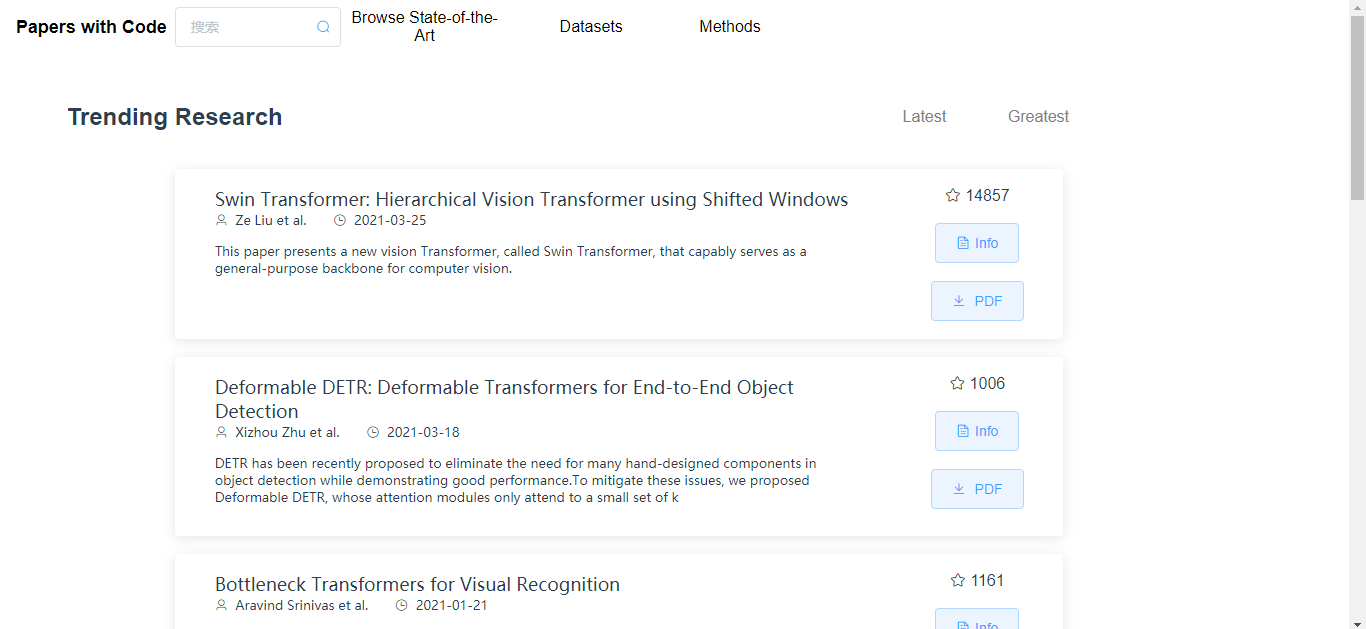
\includegraphics[width=\textwidth]{figures/main.png}
    \caption{首页}
    \label{fig:main}
\end{figure}

\begin{figure}[htbp!]
    \centering
    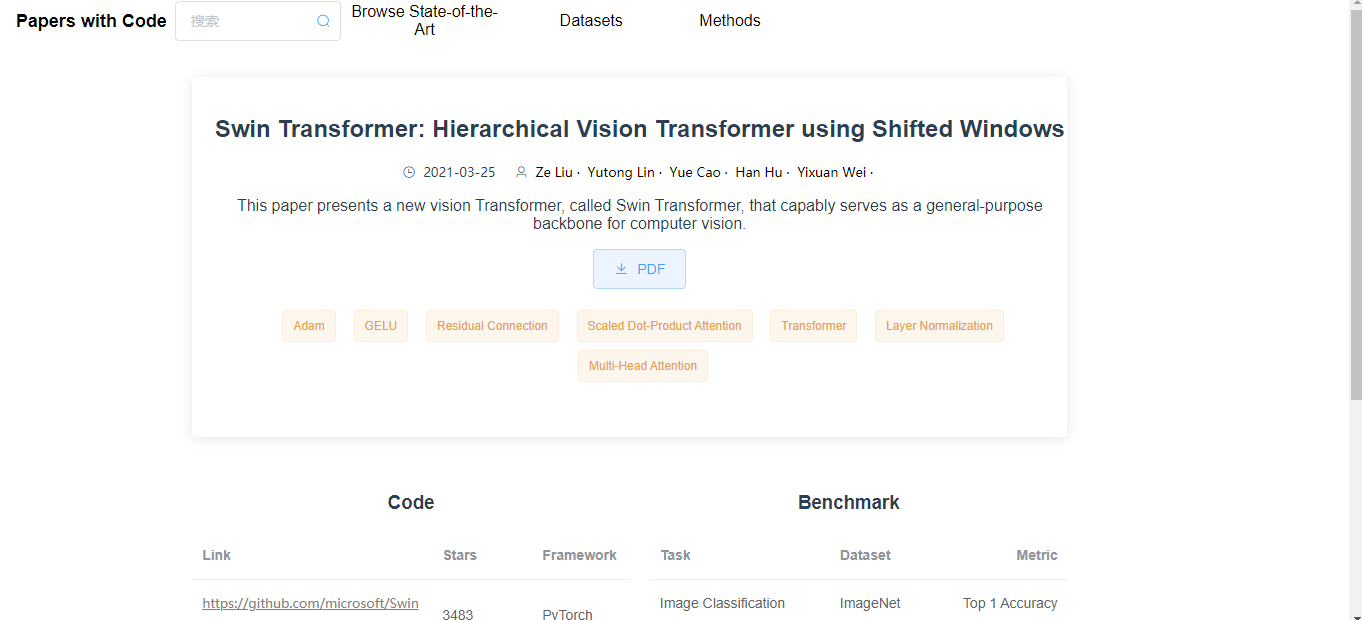
\includegraphics[width=\textwidth]{figures/paper.png}
    \caption{论文详情页}
    \label{fig:paper}
\end{figure}

\begin{figure}[htbp!]
    \centering
    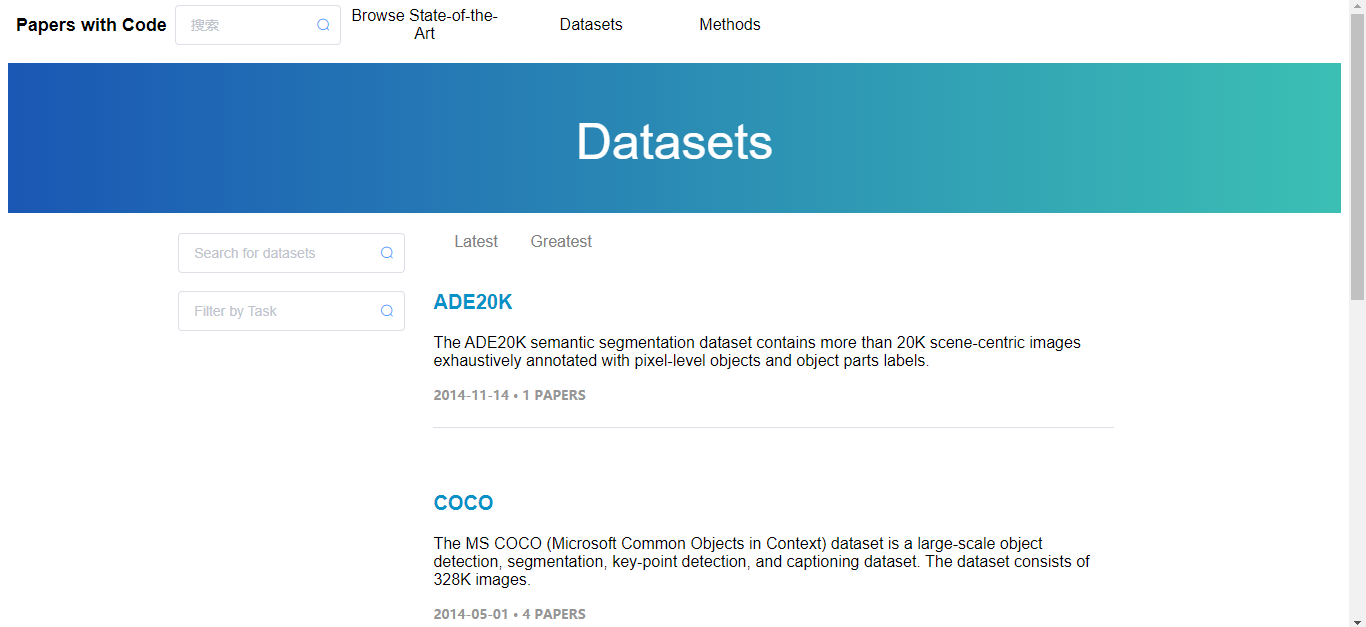
\includegraphics[width=\textwidth]{figures/dataset.png}
    \caption{数据集页}
    \label{fig:dataset}
\end{figure}

\begin{figure}[htbp!]
    \centering
    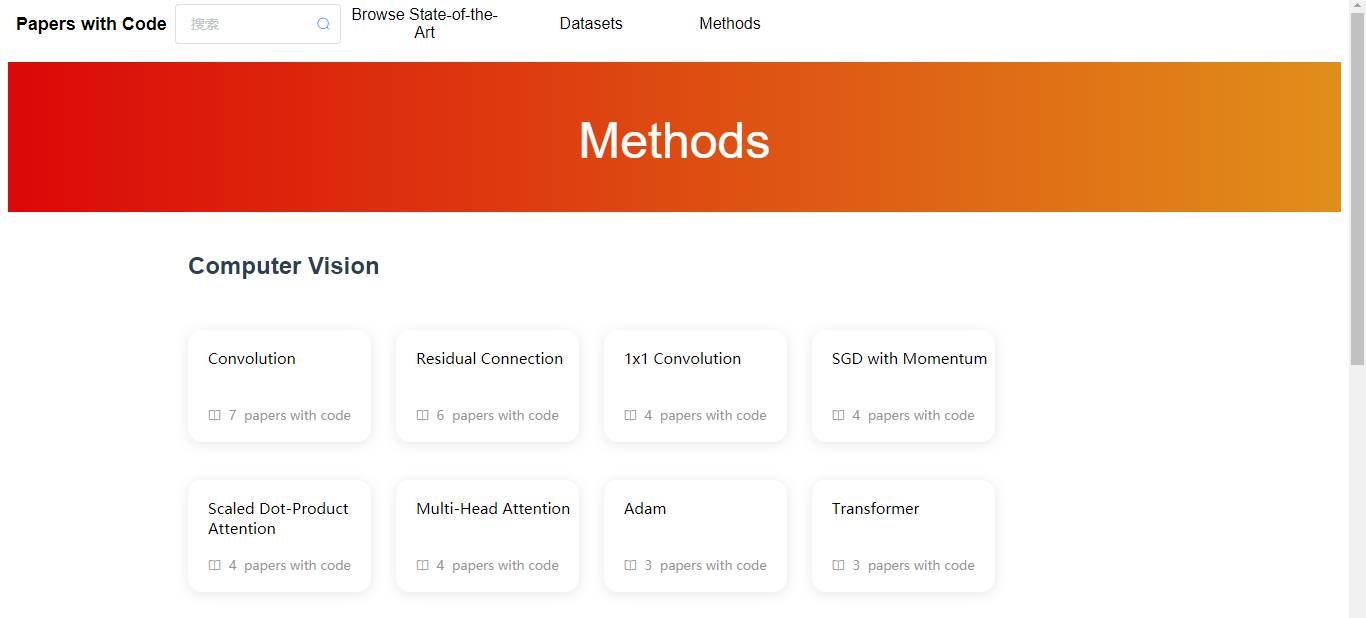
\includegraphics[width=\textwidth]{figures/method.png}
    \caption{方法页}
    \label{fig:method}
\end{figure}

\begin{figure}[htbp!]
    \centering
    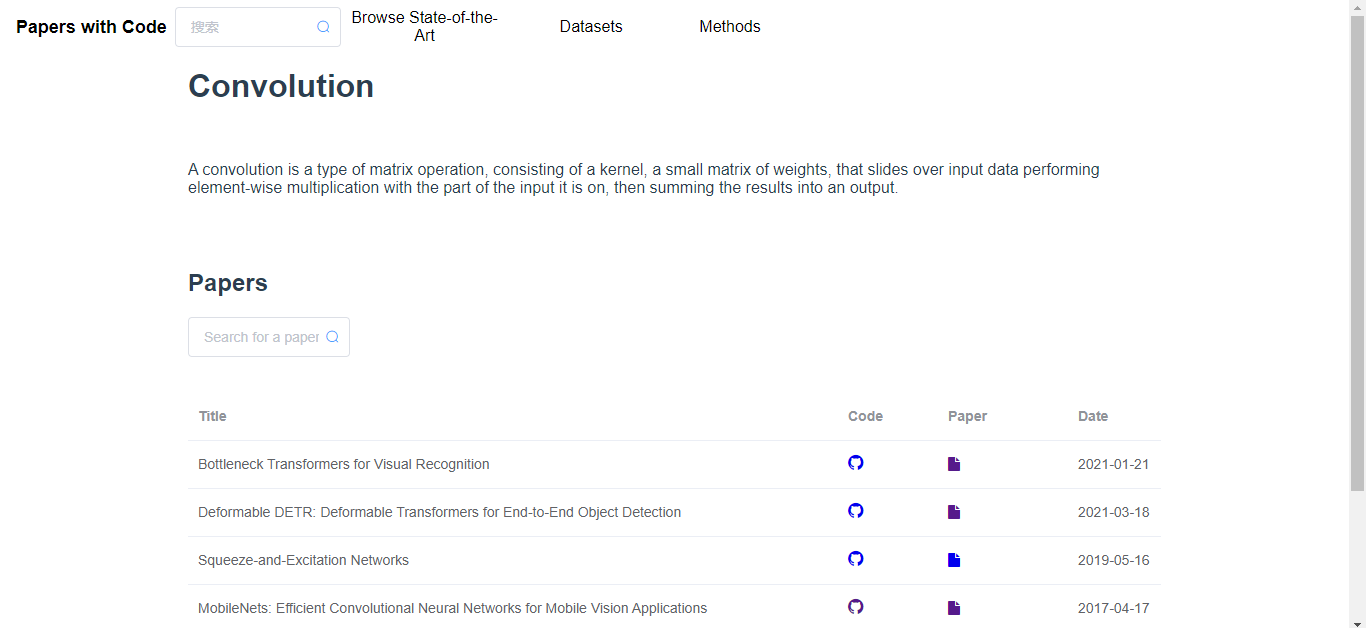
\includegraphics[width=\textwidth]{figures/methoddetail.png}
    \caption{方法详情页}
    \label{fig:methoddetail}
\end{figure}
